%!TEX program = <xelatex>
%!TEX output_directory = <K:\LaTeX>
%!TEX aux_directory = <K:\LaTeX\aux>
%!TEX jobname = <test_xelatex> 
\documentclass[12pt,a4paper]{article}
\usepackage{xeCJK}
\usepackage{latexsym}
\usepackage{amsmath}                 % AMS LaTeX宏包
\usepackage{amssymb}                 % 用来排版漂亮的数学公式
\usepackage{amsbsy}
\usepackage{amsthm}
\usepackage{amsfonts}
\usepackage{mathrsfs}                % 英文花体字体
\usepackage{bm}                      % 数学公式中的黑斜体
\usepackage{relsize}                 % 调整公式字体大小:\mathsmaller, \mathlarger
\usepackage{cmap}                   % 使pdfLatex生成的文件支持复制等
\usepackage{graphicx}                % 用于图像
\usepackage{caption}
\usepackage{setspace}                % 调节行间距
\usepackage{booktabs}                % 用于表格中加下划线
\usepackage{fancyhdr}                % 页眉页脚
\usepackage{type1cm}                 % 控制字体大小
\usepackage{indentfirst}             % 首行缩进
\usepackage{makeidx}                 % 建立索引
\usepackage{textcomp}                % 千分号等特殊符号
\usepackage{layouts}                 % 打印当前页面格式
\usepackage{bbding}                  % 一些特殊符号
\usepackage{cite}                    % 支持引用
\usepackage{minted}
% \setlength{\skip\footins}{0.5cm}     % 脚注与正文的距离
%%%%%%%%%%%%%%%%%%%%%%%%%%以上是版面控制部分%%%%%%%%%%%%%%%%%%%%%%%%%%%%%%%%%%%%%%%%%%%%%

%%%%%%%%%%%%%%%%%%%%%%%以下是版面控制部分%%%%%%%%%%%%%%%%%%%%%%%%%%%%%%%%%%%%%%%%%%%%%%
\usepackage{geometry}\geometry{left=2.75cm,right=2.5cm,top=2.5cm,bottom=2.5cm}
\usepackage{indentfirst}             % 首行缩进
\usepackage[perpage,symbol]{footmisc}% 脚注控制
\usepackage[sf]{titlesec}            % 控制标题
\usepackage{titletoc}                % 控制目录
\titlecontents{section}[0pt]{\addvspace{2pt}\filright}
              {\contentspush{\thecontentslabel\ }}
              {}{\titlerule*[8pt]{.}\contentspage}
                                     % 添加section在目录里的点号




%%%%%%%%%%%%%%%%%%%%%%%%%以下为中英文字体设置%%%%%%%%%%%%%%%%%%%%%%%%%%%%%%%%%%%%%%%%%%%
\usepackage{times}
\usepackage{fontspec,xunicode,xltxtra} % XeLaTeX相关字体字库
\XeTeXlinebreaklocale "zh"
\XeTeXlinebreakskip = 0pt plus 1pt minus 0.1pt
%\newfontfamily\youyuan{YouYuan}
%\newfontfamily\hwcaiyun{STCaiyun}
%\newfontfamily\hwhupo{STHupo}
%\newfontfamily\yaoti{FZYaoTi}
%\newfontfamily\kaiti{KaiTi_GB2312}

\newfontfamily\xsong{SimSun}
%\newfontfamily\hwsong{STSong}
% \newfontfamily\yahei{msyh.ttc}
%\newfontfamily\fangsong{FangSong_GB2312}
\newfontfamily\song{AdobeSongStd-Light}
%\newfontfamily\hwfangsong{STFangsong}
%\newfontfamily\weiti{STXinwei}
\newfontfamily\hei{AdobeHeitiStd-Regular}
\newfontfamily\kai{AdobeKaitiStd-Regular}
\newfontfamily\fsong{AdobeFangsongStd-Regular}

% \newfontfamily\cherry{CherryCreamSoda}
%\newfontfamily\hwxingkai{STXingkai}
%\newfontfamily\hwlishu{STLiti}
%\newfontfamily\zhongsong{STZhongsong}
%\newfontfamily\shuti{FZShuTi}
%\newfontfamily\hwhei{STXihei}
%\newfontfamily\lishu{LiSu}
%\newfontfamily\hwkai{STKaiti}
\newfontfamily\tnroman{Times New Roman}
\newfontfamily\consol{Consolas}
% \newfontfamily\li{jdls_s}
\newcommand{\zhIII}{\fontsize{16pt}{24pt}\selectfont}      % 三号, 1.5倍行距
\newcommand{\zhIV}{\fontsize{14pt}{21pt}\selectfont}       % 四号, 1.5倍行距
\newcommand{\zhiv}{\fontsize{12pt}{18pt}\selectfont}      % 小四, 1.5倍行距
\newcommand{\zhV}{\fontsize{10.5pt}{10.5pt}\selectfont}   % 五号, 单倍行距
\setCJKmainfont{AdobeFangsongStd-Regular}   % 设置默认中文字体



%%%%%%%%%%%%%%%%%%%%%%%%%%%%%%以下是一些命令或环境的重定义或自定义%%%%%%%%%%%%%%%%%%%%%%
\newtheorem{theorem}{定理}
\newtheorem{definition}{定义}
\newtheorem{property}{问题}
\newtheorem{proposition}{猜测}
\newtheorem{lemma}{引理}
\newtheorem{corollary}{推论}
\renewcommand{\proofname}{证明}
\renewcommand{\contentsname}{\center\hei{\zhIII{目录}}}
% \renewcommand{\refname}{\textbf{\zhiv{\song{参考文献}}}}      % 将References改为参考文献

\newenvironment{chabstract}{{\hei{\zhiv{摘要:}}}}            %定义中文摘要

\newenvironment{enabstract}{{\bfseries{\zhiv\tnroman{Abstract:}}}}         %定义英文摘要

\newenvironment{chkeyword}{{\hei{\zhiv{关键词:}}}}           %定义中文关键词

\newenvironment{enkeyword}{{\bfseries{\zhiv\tnroman{Key words:}}}}         %定义英文关键词

\newcommand{\ud}{\mathrm{d}}                                    %用\ud 作为微分算子“d”

%%%%%%%%%%%%%%%%%%%%%%%%%%%%%%以上是一些命令或环境的重定义或自定义%%%%%%%%%%%%%%%%%%%%%%%%



\setCJKmonofont{SimSun}   % 设置等宽字体
\setmainfont{MyriadPro-Regular} %设置默认英文字体。
%%%%%%%%%%%%%%%%%%%%%%%%%以上为中英文字体设置%%%%%%%%%%%%%%%%%%%%%%%%%%%%%%%%%%%%%%%%%%%




%%%%%%%%%%%%%%%%%%%%%%%以下是版面控制部分%%%%%%%%%%%%%%%%%%%%%%%%%%%%%%%%%%%%%%%%%%%%%%
\usepackage{geometry}\geometry{left=2.75cm,right=2.5cm,top=2.5cm,bottom=2.5cm}
\usepackage{indentfirst}             % 首行缩进
\usepackage[perpage,symbol]{footmisc}% 脚注控制
\usepackage[sf]{titlesec}            % 控制标题
\usepackage{titletoc}                % 控制目录

\usepackage{graphicx}
% \title{\hei{\zhIII{地图模块}}}
% \author{\li{\zhiv{忻斌健}}}
\title{\hei 地图模块}
\author{\hei 忻斌健}
\date{2017/01/09}             %本文中手动添加时间

\begin{document}
\begin{titlepage}
	\centering
	
\includegraphics[width=0.15\textwidth]{patac.jpg}\par\vspace{1cm}
	{\scshape\LARGE 泛亚汽车技术中心 \par}
	\vspace{1cm}
	{\scshape\Large 阶段性报告\par}
	\vspace{1.5cm}
	{\huge\bfseries 地图模块\par}
	\vspace{2cm}
	{\Large\itshape 忻斌健\par}
	\vfill
	协助\par
	丁稼毅\ 鞠一鸣\ 钱士才\ 李亚光

	\vfill

% Bottom of the page
	{\large \today\par}


\end{titlepage}

\clearpage                          %双面打印(openright) 用\cleardoublepage,刷新页面信息,为了添加目录章节后页码不乱
\pagenumbering{arabic}              %自此处页码开始计数
\addcontentsline{toc}{section}{\textbf{\zhiv{摘要}}} %创建虚拟章节,便于将摘要部分添加到目录
\maketitle
\begin{chabstract}
本文讨论了地图模块的接口设计和主要的功能模块以及车辆和目标在地理坐标系下的定位$\cdots$.\\
\end{chabstract}

\begin{chkeyword}
{\hei\zhiv{地图;RTK;数据融合; 路径规划;微波雷达;SRR, ESR.}}\\
\end{chkeyword}
%%%%%%%%%%%%%%%%%%%%%%%%%%%%%以上是中文摘要、关键词%%%%%%%%%%%%%%%%%%%%%%%%%%%%%%%%%



% 中图分类号:O177\\
%%%%%%%%%%%%%%%%%%%%%%%%%%%%%以下是英文题目、姓名、摘要、关键词%%%%%%%%%%%%%%%%%%%%%%%%%%%%%%%%%%%%%
\begin{center}{\bfseries{\zhIII\tnroman{HD Map implementation by RTK deployment for Path Planning with Vehicle and Object localization}}} \\
\end{center}

\begin{center}{\zhIV\tnroman{Xin Binjian}}\\
\end{center}

\begin{enabstract}\ {\zhiv\tnroman{This document has discussed the implementation of HD Map and the vehicle and objects localization in geographic coordinate system with RTK.\\}}
\end{enabstract}

\begin{enkeyword}
\ {\zhiv{HD Map;\ \ RTK;\ \ Sensor Fusion;\ \ isomorphism;\ \ Fourier transform.}}\\
\end{enkeyword}
%%%%%%%%%%%%%%%%%%%%%%%%%%%%%以上是英文题目、姓名、摘要、关键词%%%%%%%%%%%%%%%%%%%%%%%%%%%%%%%
\newpage

% \li{这是隶书}\\
% \consol{注释 test}

%%%%%%%%%%%%%%%%%%%%%%%%%%%%%以下为论文引言部分%%%%%%%%%%%%%%%%%%%%%%%%%%%%%%%%%%%%%%%%%
\section{\textbf{\zhiv{项目假设}}}

{\zhiv{\song{RTK,高精度地图,4个SRR,1个ESR;若干地标物(landmark, beacon,交通标示)
道路模型(局部地图)需要处理未知,占据和非占据信息。
接口静态的占据格栅图地图OGM+动态的目标列表。
根据静态地标占据格栅图用来更新本车姿态,叠加动态的障碍物,
局部地图:障碍物列表,车道,静态地标,RTK车辆定位--〉路径规划。}}}\\

\begin{figure}[!htb]
  \centering
  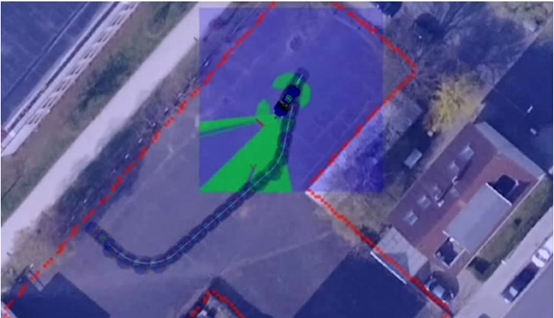
\includegraphics[height=125pt]{ogm_ex.jpg}
\end{figure}

%%%%%%%%%%%%%%%%%%%%%%%%%%%%%以上为论文引言部分%%%%%%%%%%%%%%%%%%%%%%%%%%%%%%%%%%%%%%%%%%

% \color{} 
{\zhiv{\song{

%%%%%%%%%%%%%%%%%%%%%%%%%%%%%以下为论文第二部分%%%%%%%%%%%%%%%%%%%%%%%%%%%%%%%%%%%%%%%%%%
\section{\textbf{\zhiv 2D世界模型}}

2D占据格栅图
\begin{equation}
p(m|x_{1:t},z_{1:t})=\prod_{l=1}^L p(m_l|x_{1:t},z_{1:t})
\end{equation}

\begin{figure}[!htb]
  \centering
  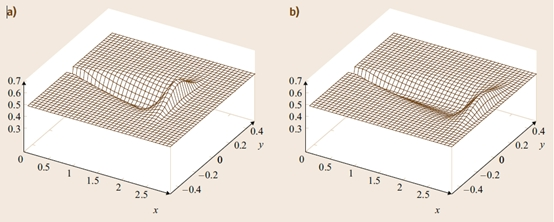
\includegraphics[height=125pt]{occupancy_prob_model.jpg}
\end{figure}


\begin{minted}[mathescape,
               linenos,
               numbersep=5pt,
               gobble=2,
               frame=lines,
               framesep=2mm]{matlab}
function [veh_pose, veh_vel] = slam_ekf_patac (innerLine, middleLine, outerLine,...
				   landmarks, ...
                   odo_motion_x, odo_motion_y, odo_motion_yaw, ...
                   rtk_gps_lat, rtk_gps_lon, rtk_gps_yaw, rtk_gps_ts,...
                   sensor_data_raw,...
                   proximity)
coder.extrinsic('EKF_prediction');    
coder.extrinsic('draw_ellipse');    
rng;%randn('state', 0);

% determines execution and display modes
coder.inline('never');
%global configuration sensor;

persistent sensor configuration step veh_origin_pose map ground; %step = 0;
%chi2 = chi2inv(configuration.alpha,1:1000);
persistent rtk_gps_lat_last rtk_gps_lon_last rtk_gps_ts_last;

if isempty(step)
    %adapt to applied sensors (SRR)!
    step = 1;

configuration = struct('ellipses',true,'tags',false,'odometry',true, ...
                        'noise',true,'alpha',0.99,'step_by_step',false,...
                        'people',false,'ground',1,'map',2,'observations',3,...
                        'compatibility',4,'ground_hypothesis',5,'hypothesis',6,...
                        'tables',7);
                    
    sensor.range = 5;
    sensor.minangle = -pi/2;
    sensor.maxangle = pi/2;
    sensor.srho = 0.01;
    sensor.stita = 0.125*pi/180;

    rtk_gps_lat_last =rtk_gps_lat;
    rtk_gps_lon_last = rtk_gps_lon;
    rtk_gps_yaw_last = rtk_gps_yaw;
    rtk_gps_ts_last = rtk_gps_ts;     
    % generate the ground data from hdmap and RTK
    ground = generate_rtk_ground(innerLine, middleLine, outerLine);

    % start with a fresh map
    [map, ground] = new_map(ground);

    % plot ground
    draw_ground(ground,landmarks, configuration);
    %%pause

    % ok, here we go

    %%observations = get_observations(ground, sensor, step);
    [x1,y1,utmzone,utmhemi] = wgs2utm(rtk_gps_lat,rtk_gps_lon,51,'N');
    veh_origin_pose.x = x1;
    veh_origin_pose.y = y1;
    veh_origin_pose.yaw = rtk_gps_yaw;
    veh_origin_pose.ts = rtk_gps_ts;
    veh_pose = veh_origin_pose;
    veh_vel = [0; 0]; % Start point with 0 velocity.
    observations = get_observations (ground, landmarks, veh_pose, ...
                                    sensor_data_raw, sensor, proximity);
    draw_observations (observations, configuration, step);
    
%     GT = zeros(1, size(sensor_data_raw,1));
%      H = zeros(1, size(sensor_data_raw,1));
    
    map = add_features(map, observations);
    % plot map
    draw_map (map, ground,configuration,step);

   % steps = length(ground.motion);
else

    step = step+1;
    disp('--------------------------------------------------------------');
%     disp(sprintf('Step: %d', step));
    
    % EKF prediction step
    odometry.x = [odo_motion_x, odo_motion_y,odo_motion_yaw]'; ;%odo_motion.x;
    odometry.P = diag([0.25 0.1 5*pi/180].^2);

   
    map = EKF_prediction (map, odometry);    

    % sense
    [x1,y1,utmzone,utmhemi] = wgs2utm(rtk_gps_lat,rtk_gps_lon,51,'N');
    veh_pose.x = x1;
    veh_pose.y = y1;
    veh_pose.yaw = rtk_gps_yaw;
    veh_pose.ts = rtk_gps_ts;

    [x2,y2,utmzone,utmhemi] = wgs2utm(rtk_gps_lat_last,rtk_gps_lon_last,51,'N');
    veh_vel = [x1-x2; y1-y2]/(rtk_gps_ts - rtk_gps_ts_last)/1000;%ms-->s

    rtk_gps_lat_last =rtk_gps_lat;
    rtk_gps_lon_last = rtk_gps_lon;
    rtk_gps_ts_last = rtk_gps_ts; 


    motion.x = [x1 y1 rtk_gps_yaw]';
    motion.P = diag([0.02 0.02 2*pi/180].^2); % expectation of std of RTK   
    ground = move_vehicle (ground, motion, step);    

    observations = get_observations(ground, landmarks, veh_pose, ...
                                    sensor_data_raw, sensor, proximity);
    
    % individual compatibility
    prediction = predict_observations (map, ground);
    compatibility = compute_compatibility (prediction, observations);

    disp(compatibility.HS);
    disp(compatibility.AL);

    disp(' ');
    
    % ground truth
    % your algorithm here!
    % 1. Try NN
    % 2. Complete SINGLES and try it
    % 3. Include people and try SINGLES5
    % 4. Try JCBB
    
    H = NN (prediction, observations, compatibility,configuration);

    draw_map (map, ground,configuration, step);
    draw_observations (observations, configuration, step);
    
    
    draw_compatibility (prediction, observations, compatibility,configuration);

    disp(' ');
    
    draw_hypothesis (prediction, observations, H, 'NN:', 'b-',configuration);

    % update EKF step
    map = EKF_update (map, prediction, observations, H, step);
    

    % only new features with no neighbours
    new = find((H == 0) & (compatibility.AL == 0));
    
    if nnz(new)
       map = add_features(map, observations, new);
    end

    draw_map (map, ground, configuration, step); 
end
veh_pose = map.x(1:3);

\end{minted}


以下给出六种典型的数列空间和函数空间的定义,文字叙述和符号表示依照文献\cite{1}.\\




\begin{definition}[空间~$l^p$   $(p\geq 1)$]               %%%%%%%%%%%%%%定义 1%%%%%%%%%%%
一切满足
~$(\sum\limits^{\infty}_{i=1}|\xi_i|^p)^{1/p}<+\infty$~    %注意命令 \limits
的数列~$x=(\xi_1,\xi_2,\cdots)$~的全体记为~$l^p$.\ 容易验证
$${\parallel x\parallel}_{p}=(\sum^{\infty}_{i=1}|\xi_i|^p)^{1/p}<+\infty$$ 是~$l^p$~上的范数.
\end{definition}
$\cdots$
%%%%%%%%%%%%%%%%%%%%%%%%以上为论文正文第二部分%%%%%%%%%%%%%%%%%%%%%%%%%%%%%%%%%%%%%%%%%%%%%%%



%%%%%%%%%%%%%%%%%%%%%%%%以下为论文正文第三部分%%%%%%%%%%%%%%%%%%%%%%%%%%%%%%%%%%%%%%%%%%%%%%
\section{\textbf{\song{\zhiv 追踪列表(动态)}}}

\begin{minted}[linenos]{c}
int main() {
printf("hello, world");
return 0;
}
\end{minted}

\begin{minted}[linenos]{c}
typedef struct{
int id;
// set to 1 in the very first cycle onl that an object is output, 0 in all other cycles.
bool newObj;
//one of GCS (WGS84/UTM), LCS,  CCS, VCS, SCS, ACS, ENUM tbd
int coordinate_system;
PatObjState objState;
PatObjSize objSize;
// Pedestrian/vehicle_car/vehicle_truck/unknown/... ---> ENUM tbd.
int objClass;
//1 if the object is moving;0 if it's still;
bool moving;
//tracking when the object is seen by which exteroceptive sensor;
PatTime lastSeenBySensor[NUM_SENSOR_EXTEROCEPTIVE];
//0 for invalid; 1 for valid;
float existenceProbability;
}PatObject;

//maximally 256 tracked objects by all sensors around the vehicle;
PatObject object_list[128];
\end{minted}

{\subsection{\textbf{\song{\zhiv{$l^p$和$L^p(\mathbf{E})$}}}}}
$l^p$~和~$L^p(\mathbf{E})$~都可分.
$\cdots$
%%%%%%%%%%%%%%%%%%%%%%%%%%%以上为论文正文第三部分%%%%%%%%%%%%%%%%%%%%%%%%%%%%%%%%%%%%%%%%%%




%%%%%%%%%%%%%%%%%%%%%%%%%%%以下为论文正文第四部分%%%%%%%%%%%%%%%%%%%%%%%%%%%%%%%%%%%%%%%%%%
{\section{\textbf{\song{\zhiv SLAM(同时定位与生成地图)}}}}

{\subsection{\textbf{\song\zhiv{函数空间与函数空间、数列空间与数列空间之间的联系}}}}


$\cdots$
{\subsection{\textbf{\song\zhiv{函数空间与数列空间的联系}}}}

\begin{lemma}[~Riesz-Fiesher~定理]                %%%%%%%%%%%%%%%%%%%%%% 引理 1 %%%%%%%%%%%%%%%%%%%%%%%%
设~$\{e_n\}$~是~Hilbert~空间~$\mathbf{H}$~中一就范正交系,$(c_1,c_2,\cdots)\in l^2$,则存在唯一的~$x\in H$~使~$(x,e_n)=e_n,\quad n=1,2,\cdots$~并且~$(x,x)=\sum\limits_{n=1}^\infty|c_n|^2$.\\
\end{lemma}


文献\cite{4}给出了~$1\leq p\leq 2$~时的~$L^p(\mathbf{E})$~上的~Fourier~变换的构造过程,并指出当
~$p>2$~时在广义函数的意义下~$L^p(\mathbf{E})$~仍可导入~Fourier~变换.\ 问题在于~$p\neq 2$~时~Fourier
~变换能否构成~$L^p(\mathbf{E})$~与~$l^p$~之间的保范同构.


\begin{property}\label{pro2}                  %%%%%%%%%%%%%%%%% 问题 2 %%%%%%%%%%%%%%%%%%%%%%%%
完备距离空间~$S(\mathbf{E})$~与~$s$,Banach~空间~$M(\mathbf{E})$~与~$m$~之间是否有同构关系?更进一步,~Fourier~变换及其反演公式
能否推广到完备距离空间~$S(\mathbf{E})$~与~$s$,Banach~空间~$M(\mathbf{E})$~ 与~$m$
\end{property}
%%%%%%%%%%%%%%%%%%%%%%%%%以上是论文正文的第四部分%%%%%%%%%%%%%%%%%%%%%%%%%%%%%%%%%%%%%%%%%%%%
}}}


%%%%%%%%%%%%%%%%%%%%%%%%%以下是参考文献%%%%%%%%%%%%%%%%%%%%%%%%%%%%%%%%%%%%%%%%%%%%%%%%

\clearpage %双面打印(openright) 用\cleardoublepage
\addcontentsline{toc}{section}{\textbf{\zhiv{参考文献}}}
\begin{thebibliography}{99}
{\song{\zhV
\bibitem{1}那汤松.\ 实变函数论(第5版).\ 徐瑞云 译.\ 北京:高等教育出版社,2010.
\bibitem{2}郭大钧等.\ 实变函数与泛函分析(第二版)$\cdot$ 下册.\ 山东:山东大学出版社,2005.
\bibitem{3}夏道行等.\ 实变函数论与泛函分析(下册$\cdot$ 第二版修订本).\ 北京:高等教育出版社,2010.
\bibitem{4}A.H.柯尔莫戈洛夫,C.B.佛明.\ 函数论与泛函分析初步(第7 版).\ 北京:高等教育出版社,2006.
}
}
\end{thebibliography}

\end{document}